%Preamble
\documentclass[newPxFont]{beamer}
\usetheme{sthlm}
%\usecolortheme{sthlmv42}
%-=-=-=-=-=-=-=-=-=-=-=-=-=-=-=-=-=
%        Packages
%-=-=-=-=-=-=-=-=-=-=-=-=-=-=-=-=-=
\usepackage[utf8]{inputenc}
\usepackage{chronology}
\usepackage{hyperref}
\usepackage{amsmath}
\usepackage{amssymb}
\usepackage{booktabs}
%----------------------------------
%Comandos:
\newcommand \imageFrame[2]{
\begingroup
\begin{frame}
  \begin{center}
\includegraphics[width=4in]{#1}\\
\Large #2
    \end{center}
\end{frame}
\endgroup
}

\renewcommand{\event}[3][e]{%
  \pgfmathsetlength\xstop{(#2-\theyearstart)*\unit}%
  \ifx #1e%
    \draw[fill=black,draw=none,opacity=0.5]%
      (\xstop, 0) circle (.2\unit)%
      node[opacity=1,rotate=45,right=.2\unit] {#3};%
  \else%
    \pgfmathsetlength\xstart{(#1-\theyearstart)*\unit}%
    \draw[fill=black,draw=none,opacity=0.5,rounded corners=.1\unit]%
      (\xstart,-.1\unit) rectangle%
      node[opacity=1,rotate=45,right=.2\unit] {#3} (\xstop,.1\unit);%
  \fi}%
%-=-=-=-=-=-=-=-=-=-=-=-=-=-=-=-=-=-=-
%        Beamer options
%-=-=-=-=-=-=-=-=-=-=-=-=-=-=-=-=-=-=-%\setbeameroption{show notes}
%-=-=-=-=-=-=-=-=-=-=-=-=-=-=-=-=-=-=-
%
%	Information
%
%-=-=-=-=-=-=-=-=-=-=-=-=-=-=-=-=-=-=-
\title{Biomedical Engineering Summer School, Wilhelmshaven 2018}
\subtitle{ Instrumentation, Acquisition and Signal Processing for Biosignals}
%\date{\small{\jobname}}
\date{\today}
\author{\texttt{Gerardo Marx Chávez-Campos\\ Mehmet Y\"uksekkaya}}
\institute{\textit{Instituto Tecnológico de Morelia}}


\hypersetup{
pdfauthor = {Marx: gmarx-cc@itmorelia.edu.mx},
pdfsubject = {Fourier series},
pdfkeywords = {orthogonal function, },
pdfmoddate= {D:\pdfdate},
pdfcreator = {Chavez-Campos}
}

\begin{document}
%Title:
\maketitle
%\begin{frame}[plain]
%	\titlepage
%\end{frame}
\begin{frame}{Contest}
\tableofcontents[]
\end{frame}


%=-=-=-=-=-=-=-=-=-=-=-=-=-=-=-=-
\section{Sequence of numbers}
%=-=-=-=-=-=-=-=-=-=-=-=-=-=-=-=-
%=-=-=-=-=-=-=-=-=-=-=-=-=-=-=-=-
\begin{frame}{Sequence of numbers}
\begin{itemize}
  \item Numbers have been used to represent things and count it.
  \item The counting activity allows to know ``How many?''
\end{itemize}

\begin{figure}
  
\includegraphics[width=3in]{history_of_numbers_by_buzzios}
\end{figure}
\end{frame}
%=-=-=-=-=-=-=-=-=-=-=-=-=-=-=-=-
\begin{frame}
\begin{itemize}
  \item However, human beings observe that numbers are in nature in specific sequences\cite{Nova2017}...
\end{itemize}

\begin{figure}
  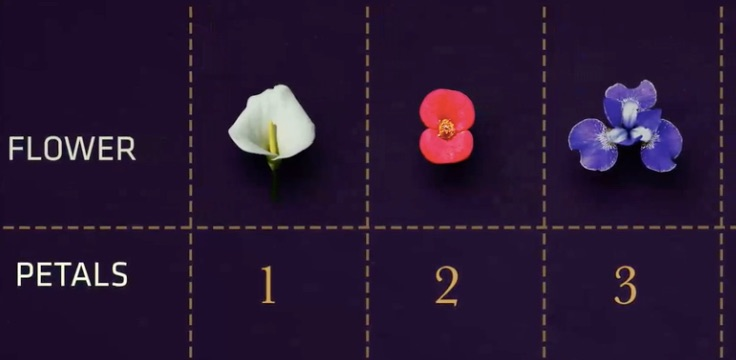
\includegraphics[width=4in]{fibonacci1}
\end{figure}
\end{frame}
%=-=-=-=-=-=-=-=-=-=-=-=-=-=-=-=-
\begin{frame}
\begin{figure}
  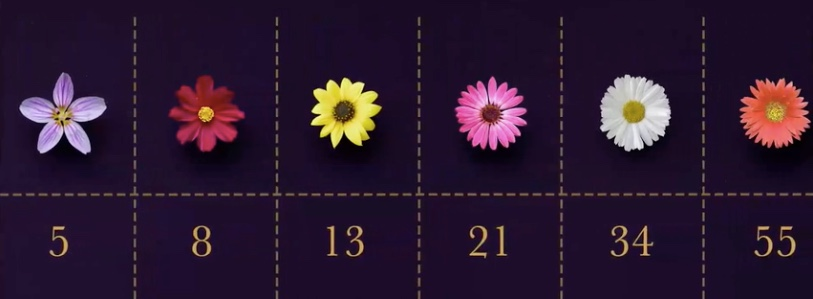
\includegraphics[width=4.3in]{fibonacci2}
\end{figure}
\end{frame}
%=-=-=-=-=-=-=-=-=-=-=-=-=-=-=-=-
\begin{frame}
Let's take a look to this sequence:
\begin{itemize}
  \item 1
  \item 2
  \item 3
  \item 5
  \item 8
  \item 13
  \item 21
  \item 34
  \item 55
  \item ... and so on
\end{itemize}
Can you find some way to relate this numbers?
\end{frame}
%=-=-=-=-=-=-=-=-=-=-=-=-=-=-=-=-
\imageFrame{pine1}{How many spirals can you count?}
%=-=-=-=-=-=-=-=-=-=-=-=-=-=-=-=-
\imageFrame{pine}{The same sequence...}
%%=-=-=-=-=-=-=-=-=-=-=-=-=-=-=-=-
\begin{frame}{The Fibonacci sequence}
The \alert{Fibonacci} sequence is widely found in most nature phenomena. The sequence is easily to create it by the sum of the previos terms:
\begin{eqnarray*}
  u_0=0\\
  u_1=1\\
  u_2=u_0+u_1=0+1=1\\
  u_3=u_1+u_2=1+1=2\\
  u_4=u_2+u_3=2+1=3\\
  %u_5=u_3+u_4=2+3=5\\
  \vdots\\
  u_n=u_{n-1}+u_{n-2}
\end{eqnarray*}
\end{frame}
%=-=-=-=-=-=-=-=-=-=-=-=-=-=-=-=-
\begin{frame}{What is a sequence?}
  \begin{block}{Sequence definition}
    A \textbf{sequence} is a list of things (usually numbers) that are in order:\\
    \begin{equation}
          \underbrace{3}_{\text{1st term}},\underbrace {5}_{\text{2nd term}} ,\underbrace {7}_{\text{3rd term}},\underbrace {9}_{\text{4th term}},\hdots, \underbrace{n}_{\text{nth term}}
    \end{equation}
  \end{block}
  \pause
  A sequence is usually defined by a \alert{Rule}, this is a way or equation to find each term\cite{Math2017}. Thus, in order to be able of determine ($u_n$, $n$th term) the \alert{Rule} is written as a formula, where $n$ is any term.
\end{frame}
%=-=-=-=-=-=-=-=-=-=-=-=-=-=-=-=-
\begin{frame}
    Then, the \alert{Rule} for the sequence $\{ 3,5,7,9,\hdots,\infty\}$ is:
    \begin{table}
      \begin{tabular}{ccc}
     $n$ &\bfseries Term &\bfseries Test rule \\\toprule
     1 & 3 & $2\times 1 +1=3$\\
     2 & 5 & $2\times 2 +1=5$\\
     3 & 7 & $2\times 3 +1=7$\\
     \bottomrule
     \end{tabular}
    \end{table}
\end{frame}
%=-=-=-=-=-=-=-=-=-=-=-=-=-=-=-=-
\begin{frame}{Special sequences}
  \begin{itemize}
    \item <1-> \alert{Arithmetic} sequence has a \alert{constant} value between one term and other e.g. $\{1,4,7,10,13,\hdots\}$, write as an equation: $a_n=a_1+(n-1)d$.
    \item <2-> In the \alert{Geometric} sequence each term is found by multiplying the previous term by a \alert{constant} value: $\{2,4,8,16,32,\hdots,\}$, as an equation:  $a_n=a_1\cdot r^{n-1}$.
    \item <3-> The \alert{Triangular} sequence is generated from dots patterns that form triangles: $\{1,3,6,10,15,21,\}= n(n+1)/2$.
  \end{itemize}
  \visible<4->{\begin{figure}
    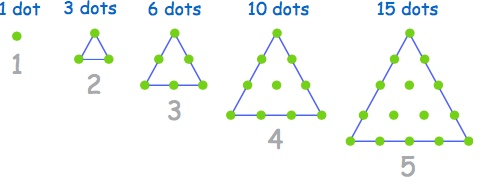
\includegraphics[width=2.5in]{triangular}
  \end{figure}}
\end{frame}
%=-=-=-=-=-=-=-=-=-=-=-=-=-=-=-=-
%Here I am @jade
\imageFrame{exer1}{Matlab time...}
%=-=-=-=-=-=-=-=-=-=-=-=-=-=-=-=-
\section{Series}
\imageFrame{netflix}{No, no this kind of series...}
%=-=-=-=-=-=-=-=-=-=-=-=-=-=-=-=-
\begin{frame}{Finite and infinite series}
  \begin{block}{Finite Series}
    Let ${u_n}$ be a sequence. Then the finite sum (partial sum) order is:\\
    \begin{equation}
        S_n=u_1+u_2+u_3+\hdots+u_n
    \end{equation}
  \end{block}
  \pause
  \begin{block}{Infinite Series}
    Let ${u_n}$ be a sequence. Then the Infinite sum order is:\\
    \begin{equation}
        \sum_{n=1}^\infty u_n=u_1+u_2+u_3+\hdots
    \end{equation}
  \end{block}
\end{frame}
%=-=-=-=-=-=-=-=-=-=-=-=-=-=-=-=-
%=-=-=-=-=-=-=-=-=-=-=-=-=-=-=-=-
\begin{frame}{The $n_{th}$ term theorem}
If the partial sums $S_n$ converge to $L$ as $n\longrightarrow \infty$, we can say that the infinite series converges to $L$\cite{Math242017}.

\begin{theorem}
If
\begin{equation}
  \lim_{n \to +\infty} U_n=0\label{eq:kthterm}
\end{equation}
the infinity series $\sum_{n=1}^{+\infty} U_n$ is \alert{convergent}
\vspace{0.2in}\\
If
\begin{equation}
  \lim_{n \to +\infty} U_n\neq0
\end{equation}
the infinity series $\sum_{n=1}^{+\infty} U_n$ is \alert{divergent}
\end{theorem}
\end{frame}
%=-==-==-==-==-==-==-==
\imageFrame{L}{A convergent series}
%=-==-==-==-==-==-==-==
\begin{frame}{Does the harmonic series converges?}
Note that the Theorem \eqref{eq:kthterm} not always is true. In other words, it is possible to have a \alert{divergent} series for which $\lim_{n \to +\infty} U_n=0$. An example of such a series is the one known as the harmonic, which is

\pause
\begin{equation}
  \sum_{n=1}^{+\infty} \frac{1}{n}=1+\frac{1}{2}+\frac{1}{3}+\frac{1}{4}+\frac{1}{5}+\frac{1}{6}\cdots+\frac{1}{n}\cdots
\end{equation}
\end{frame}
%=-==-==-==-==-==-==-==
\imageFrame{harmonic}{The harmonic series}
%=-==-==-==-==-==-==-==
\begin{frame}{Infinite series of constant terms}
Giving the infinite series :
\begin{eqnarray*}
  \sum_{n=1}^\infty \frac{1}{n(n+1)}\\\pause
  s_1=u_1=\frac{1}{1\cdot2}=\frac{1}{2}\\\pause
  s_2=s_1+u_2=\frac{1}{2}+\frac{1}{2\cdot3}=\frac{2}{3}\\\pause
  s_3=s_2+u_3=\frac{2}{3}+\frac{1}{3\cdot4}=\frac{3}{4}\\\pause
  s_4=s_3+u_3=\frac{3}{4}+\frac{1}{4\cdot5}=\frac{4}{5}\\
\end{eqnarray*}
\end{frame}
%=-==-==-==-==-==-==-==
\begin{frame}
using partial fractions, it is more evident to see that
\begin{eqnarray*}
  u_k=\frac{1}{k(k+1)}=\frac{1}{k}-\frac{1}{k+1}\\
  \end{eqnarray*}
  Therefore
  \begin{eqnarray*}
  s_n=\left(1-\frac{1}{2}\right)+\left(\frac{1}{2} -\frac{1}{3}\right)+\left(\frac{1}{3} -\frac{1}{4}\right)+\hdots\\+ \left(\frac{1}{n-1} -\frac{1}{n}\right)+ \left(\frac{1}{n} -\frac{1}{n+1}\right)
  \end{eqnarray*}
  Removing the opposite terms, we have
  \begin{eqnarray*}
  s_n=1-\frac{1}{n+1}=\frac{n}{n+1}
\end{eqnarray*}
\end{frame}
%=-==-==-==-==-==-==-==
\imageFrame{exer2}{Do your own code for a series..}
%=-==-==-==-==-==-==-==
\begin{frame}{More test are required}
Therefore, considering the possibilities in sequences, hence in series, more ways to know if a series  \alert{converges} or \alert{diverges} are needed.
\end{frame}
%=-==-==-==-==-==-==-==
\subsection{The integral test}
\begin{frame}{The integral test}
%The theorem known as the \alert{integral test} makes use of the theory of improper integrals to test an infinite series of positive terms for convergence.
\begin{theorem}
    Let $f$ be a function which is continuous, decreasing, and positive valued for all $x>=1$, then the infinite series
    \begin{equation*}
      \sum_{n=1}^{+\infty} f(n)=f(1)+f(2)+\cdots+f(n)+\cdots
    \end{equation*}
    is \alert{convergent} if the improper integral
    \begin{equation*}
      \int_1^{+\infty} f(x)dx
    \end{equation*}
    exists, and is \alert{divergent} if the improper integral increase without bound.
  \end{theorem}
\end{frame}
%=-=-=-=-=-=-=-=-=-=-=-=-=-=-=-
\subsection{The ratio test}
\begin{frame}
  \begin{theorem}
    Let $\sum a_n$ be an infinite series of nonzero terms and let $L$ to be calculated by \eqref{eq:ratio}
    \begin{equation}
        \lim_{n\to+\infty} \left|\frac{a_{n+1}}{a_n}\right|=L\label{eq:ratio}
      \end{equation}
thus:
\pause
    \begin{itemize}
      \item If $L<1$, the series is absolutely convergent. \pause
      \item If $L>1$, or $L\to\infty$, the series is divergent. \pause
      \item If $L=1$, the series may be absolutely convergent, conditionally convergent, or divergent.
    \end{itemize}
        \end{theorem}
\end{frame}
%=-==-==-==-==-==-==-==-==-==-=


\section{Power series}
\begin{frame}{Power series}
\begin{theorem}
  Let $x$ be a variable. \alert{A power series in $x$} is a series of the form:
  \begin{equation}
    \sum_{n=0}^{\infty} a_n x^n=a_0+a_1 x+a_2 x^2+\cdots+a_n x^n+\cdots
  \end{equation}
  where each $a_n$ is a real number\cite{Swokowski1983}.
\end{theorem}
\end{frame}
%=-==-==-==-==-==-==-==-==-==-=
\imageFrame{exercise}{Exercise time..}
%=-==-==-==-==-==-==-==-==-==-=
\begin{frame}{Exercise:}
  Find all values of $x$ for which the following power series is absolutely convergent:
  \begin{eqnarray}
    1+\frac{1}{5}x+\frac{2}{5^2}x^2+\cdots+\frac{n}{5^n}x^n+\cdots
  \end{eqnarray}
  \alert{use the ratio test!}
\end{frame}
%=-==-==-==-==-==-==-==-==-==-=
\imageFrame{geometryc}{convergency radius}
%=-==-==-==-==-==-==-==-==-==-=
\subsection{Power series convergency}
\begin{frame}{Power series convergency theorem}
\begin{theorem}
  If $\sum a_n x^n$ is a power series, then precisely one of the following is true
  \begin{itemize}
    \item The series converges only if $x=0$,
    \item The series is absolutely convergent for all $x$,
    \item There is a positive number $r$ such that the series is absolutely convergent if $|x|<r$ and divergent if $|x|>r$
  \end{itemize}
\end{theorem}
\end{frame}
%=-=-==-=-==-=-==-=-==-=-==-=-==-=-=
\begin{frame}{Power series $(x-c)$}
\begin{theorem}
  Let $c$ be a real number and $x$ a variable. \alert{A power series in} $(x-c)$ is a series of the form
  \begin{equation}
    \sum_{n=0}^{+\infty}a_n (x-c)^n=a_0+a_1(x-c)+a_2(x-c)^2+\cdots+a_n(x-c)^n+\cdots
  \end{equation}
  where each $a_n$ is a real number.
\end{theorem}
\end{frame}
%=-==-==-==-==-==-==-==-==-==-=
\imageFrame{geometryc2}{convergency radius}
%=-==-==-==-==-==-==-==-==-==-=
\subsection{Power series representations of functions}
\begin{frame}{Power series representations of functions}
  A \alert{power series} $\sum a_nx^n$ can be used to define a function of $f(x)$ whose domain is the interval of convergence of the series. Specifically, for each $x$ in this interval we let $f(x)$ equal the sum of the series, that is
  \begin{equation}
    f(x)=a_0+a_1x+a_2x^2+\cdots+a_nx^n+\cdots
  \end{equation}
If a function $f(x)$ is defined in this way we say that $\sum a_nx^n$ is \alert{a power series representative for $f(x)$}.

\alert{This allows us to find values in a new way}. Specifically, if $c$ is the interval of convergence, thus $f(c)$ can be found  or approximated ($\simeq$) be the series.
\end{frame}
%=-==-==-==-==-==-==-==-==-==-=
\subsection{Derivatives and integrals}
\begin{frame}{Derivatives}
  \begin{theorem}
    Suppose a power series $\sum a_nx^n$ has a nonzero radius of convergence $r$ and let the function $f$ be defined by
    \begin{equation}
      f(x)=\sum_{n=0}^{\infty}a_nx^n\label{eq:powerSeries}
    \end{equation}
for every $x$ in the interval of convergence. If $-r<x<r$, then:
    \begin{eqnarray}
      f'(x)=\sum_{n=0}^{\infty}D_x(a_nx^n)=\sum_{n=1}^\infty na_nx^{(n-1)}\label{eq:derivative}\\\nonumber
      =a_1+2a_2x+3a_3x^2+\cdots+na_nx^{(n-1)}+\cdots
    \end{eqnarray}
  \end{theorem}
\end{frame}
%=-==-==-==-==-==-==-==-==-==-=
\begin{frame}{Integral}
\begin{theorem}
\begin{eqnarray}
  \int_0^x f(t)dt=\sum_{n=0}^{\infty}\int_0^x (a_nt^n)dt=\sum_{n=0}^\infty \frac{a_n}{n+1}x^{n+1}\label{eq:integral}\\\nonumber
  =a_0x+\frac{1}{2}a_1x^2+\frac{1}{3}a_2x^3+\cdots+\frac{1}{n+1}a_nx^{n+1}+\cdots
\end{eqnarray}
\end{theorem}
  \begin{alertblock}{to consider}
    as can be shown in Equations \eqref{eq:derivative} and \eqref{eq:integral} the convergency radius remains equal to \eqref{eq:powerSeries}.
  \end{alertblock}
\end{frame}
%=-==-==-==-==-==-==-==-==-==-=
%\begin{frame}{Exercise:}
%  Prove that :
%  \begin{eqnarray}
%    1+\frac{1}{5}x+\frac{2}{5^2}x^2+\cdots+\frac{n}{5^n}x^n+\cdots
%  \end{eqnarray}
%  \alert{use the ratio test!}
%\end{frame}
%=-==-==-==-==-==-==-==-==-==-=
%=-=-==-=-==-=-==-=-==-=-==-=-==-=-=
\section{Tylor and Maclaurin Series}
\begin{frame}{Tylor and Maclaurin Series}
  Suppose a function $f$ is represented by a power series in $x-c$, such that
  \begin{equation}
    f(x)=\sum_{n=0}^{+\infty}a_n (x-c)^n=a_0+a_1(x-c)+a_2(x-c)^2+a_3(x-c)^3+\cdots
  \end{equation}
where the domain of $f$ is an open interval containing $c$
\end{frame}

\begin{frame}
  \begin{eqnarray}
    f'(x)=\sum_{n=1}^\infty na_n(x-c)^{n-1}\\\nonumber
    =a_1+2a_2(x-c)+3a_3(x-c)^2+4a_4(x-c)^3+\cdots\\
    f''(x)=\sum_{n=2}^\infty n(n-1)a_n(x-c)^{n-2}\\\nonumber
    =2a_2+(3\cdot2)a_3(x-c)+(4\cdot3)a_4(x-c)^2+\cdots\\
    f'''(x)=\sum_{n=3}^\infty n(n-1)(n-2)a_n(x-c)^{n-3}\\\nonumber
    =(3\cdot2)a_3+(4\cdot3\cdot2)a_4(x-c)+\cdots
  \end{eqnarray}
\end{frame}

\begin{frame}
  and, for every positive integer $k$,
  \begin{eqnarray}
    f^{(k)}(x)=\sum_{n=k}^{\infty} n(n-1)\cdots(n-k+1)a_n(x-c)^{n-k}
  \end{eqnarray}
  Moreover, each series obtained by differentiation has the same radius of convergence as the original series. Substituting $c$ for $x$ in each of these series representation, we obtain
  \begin{eqnarray}
    f(c)=a_0\\
    f'(c)=a_1\\
    f''(c)=2a_2\\
    f'''(c)=(3\cdot2)a_3\\
    f^{(n)}(c)=n!a_n \to a_n=\frac{f^{(n)}(c)}{n!}
  \end{eqnarray}
\end{frame}

\begin{frame}{Taylor series}
\begin{theorem}
  If $f$ is a function and
  \begin{equation}
    f(x)=\sum_{n=0}^\infty a_n(x-c)^n
  \end{equation}
  for all $x$ in an open interval containing $c$, then
  \begin{equation}
    f(x)=f(c)+f'(c)(x-c)+\frac{f''(c)}{2!}(x-c)^2+\cdots+\frac{f^{(n)}(c)}{n!}(x-c)^n
  \end{equation}
\end{theorem}
\end{frame}

\begin{frame}{Maclaurin}
  \begin{Corollary}
    If $f$ is a function and $f(x)=\sum a_nx^n$ for all $x$ in an open interval $(-r,r)$, then
    \begin{equation}
    f(x)=f(0)+f'(0)x+\frac{f''(0)}{2!}x^2+\cdots+\frac{f^{(n)}(0)}{n!}x^n+\cdots
    \end{equation}
  \end{Corollary}
\end{frame}

%=-==-==-==-==-==-==-==-==-==-=
%=-==-==-==-==-==-==-==-==-==-=
%=-==-==-==-==-==-==-==-==-==-=
%=-==-==-==-==-==-==-==-==-==-=
%=-==-==-==-==-==-==-==-==-==-=
%=-==-==-==-==-==-==-==-==-==-=
%=-==-==-==-==-==-==-==-==-==-=
%=-==-==-==-==-==-==-==-==-==-=

%\begin{frame}{Introduction}
%
%The concepts of geometric vectors in two and three dimensions, orthogonal or perpendicular vectors, and the inner product of two vectors have been generalized. It is perfectly routine in mathematics to think of a function as a vector. In this section we will examine an \alert{inner product that is different from the one you studied in calculus}. Using this new inner product, we define \alert{orthogonal functions and sets of orthogonal functions}. Another topic in a standard calculus course is the expansion of a function $f$ in a power series. In this section we will also see how to expand a suitable function $f$ in terms of an infinite set of orthogonal functions.\cite{Zill2009}
%\end{frame}
%%=-=-=-=-=-=-=-=-=-=-=-=-=-=-=-=-
%\subsection{Inner product}
%\begin{frame}{Inner product}
%Recall that if $u$ and $v$ are two vectors in 3-space, then the inner product $(u, v)$ (in calculus this is written as $u\cdot v$) possesses the following properties:
%  \pause
%  \begin{block}{Inner product definitions}
%    \begin{enumerate}
%        \item $(u,v)=(v,u)$
%        \item $(ku,v)=k(u,v)$, $k$ is a scalar
%        \item $(u,u)=0$ if $u=0$ and $(u,u)>0$ if $u\neq0$
%        \item $(u+v,w)=(u,w)+(v,w)$
%    \end{enumerate}
%\end{block}
%\end{frame}
%%=-=-=-=-=-=-=-=-=-=-=-=-=-=-=-=-
%\begin{frame}{Inner product cont...}
%\begin{definition}[Inner product of functions]
%  The \alert{inner product} of two functions $f_1$ and $f_2$ on an interval $[a, b]$ is the number
%  \begin{equation}
%    (f_1,f_2)=\int_a^b f_1(x)f_2(x)dx
%  \end{equation}
%\end{definition}
%\end{frame}
%%=-=-=-=-=-=-=-=-=-=-=-=-=-=-=-=-
%\subsection{Orthogonal function definition}
%\begin{frame}{Inner product cont...}
%\begin{definition}[Orthogonal functions]
%  Two functions $f_1$ and $f_2$ are \alert{orthogonal} on an interval $[a, b]$ if
%  \begin{equation}
%    (f_1,f_2)=\int_a^b f_1(x)f_2(x)dx=0\label{eq:orthogonal}
%  \end{equation}
%\end{definition}
%\end{frame}
%%=-=-=-=-=-=-=-=-=-=-=-=-=-=-=-=-
%\subsection{Example}
%\begin{frame}{Example}
%  \begin{exampleblock}{Exercise 1}
%    Consider $f_1=x^2$ and $f_2=x^3$. Determine if functions are orthogonal on interval [-1,1]:
%  \end{exampleblock}
%  \pause
%  %resolución
%  \begin{alertblock}{Warning}
%  Unlike in vector analysis, in which the word orthogonal is a synonym for perpendicular, in this present context the term orthogonal and condition \eqref{eq:orthogonal} have no geometric significance.
%  \end{alertblock}
%\end{frame}
%%=-=-=-=-=-=-=-=-=-=-=-=-=-=-=-=-
%\subsection{Orthogonal sets}
%\begin{frame}{Orthogonal sets}
%We are  primarily interested in infinite sets of orthogonal functions.
%
%\begin{definition}[Orthogonal Set]
%  A set of real-valued functions $\lbrace{\phi_0(x), \phi_1(x), \phi_2(x),\dots\rbrace}$ is said to be orthogonal on an interval $[a, b]$ if
%  \begin{equation}
%    (\phi_m,\phi_n)=\int_a^b \phi_m(x)\phi_n(x)dx=0, \; m\neq n
%  \end{equation}
%\end{definition}
%\end{frame}
%%=-=-=-=-=-=-=-=-=-=-=-=-=-=-=-=-
%\begin{frame}{The norm or length}
%The norm, or length  $||u||$ , of a vector $u$ can be expressed in terms of the inner product. The expression $(u, u)=||u||^2$ is called the square norm, and so the norm is $||u||=\sqrt{(u, u)}$.
%\pause
%\vspace{1em}
%
% Similarly, the square norm of a function $\phi_n$ is  $||\phi_n(x)^2||=(\phi_n,\phi_n)$, and so the \alert{norm}, or its generalized length, is  $||\phi_n(x)||=\sqrt{(\phi_n,\phi_n)}$. In other words, the square norm and norm of a function $\phi_n$ in an orthogonal set $\lbrace{\phi_n(x)\rbrace}$ are, respectively,
%\end{frame}
%%=-=-=-=-=-=-=-=-=-=-=-=-=-=-=-=-
%\begin{frame}{Orthonormal sets}
%\begin{equation}
%  ||\phi_n(x)||^2=\int_a^b \phi_n^2(x)dx
%\end{equation}
%and
%\begin{equation}
%  ||\phi_n(x)||=\sqrt{\int_a^b\phi_n^2(x)dx}
%\end{equation}
%\pause
%If $\lbrace{\phi_n(x)\rbrace}$ is an orthogonal set of functions on the interval $[a, b]$ with the property that  $\phi_n(x)=1$ for $n=0, 1, 2,...,$ then ${\phi_n(x)}$ is said to be an \alert{orthonormal set} on the interval.
%\end{frame}
%%=-=-=-=-=-=-=-=-=-=-=-=-=-=-=-=-
%\begin{frame}{Examples}
%  \begin{exampleblock}{Exercise 2}
%    Show that the set $\lbrace{1, cos(x), cos(2x),\dots\rbrace}$ is orthogonal on the interval $[-\pi,\pi]$.
%  \end{exampleblock}
%  \pause
%  %Resolution
%
%\end{frame}
%%=-=-=-=-=-=-=-=-=-=-=-=-=-=-=-=-
%\begin{frame}{Examples...}
%  \begin{exampleblock}{Exercise 3}
%    Find the norm of each function in the orthogonal set given in Example 2.
%  \end{exampleblock}
%  %Resolution
%  \pause
%  \begin{itemize}
%    \item Find $||\phi_0(x)||$
%    \item Find $||\phi_n(x)||$
%  \end{itemize}
%  \pause
%Any orthogonal set of nonzero functions $\lbrace{\phi_n(x)\rbrace}$, $n=0, 1, 2,\dots$ can be \alert{normalized} -that is, made into an orthonormal set- by dividing each function by its norm. It follows from Examples 2 and 3 that the set is
%\end{frame}
%%=-=-=-=-=-=-=-=-=-=-=-=-=-=-=-=-
%\begin{frame}{Exercise 3 conclusion}
%\begin{equation}
%   \biggl\lbrace \frac{1}{\sqrt{2\pi}},\frac{cos(x)}{\sqrt{\pi}},\frac{cos(2x)}{\sqrt{\pi}},\dots\biggr\rbrace
%\end{equation}
%is orthonormal on the interval $[\pi,-\pi]$.
%\end{frame}
%%=-=-=-=-=-=-=-=-=-=-=-=-=-=-=-=-
%\imageFrame{bartFourier}{Time for a meme ;)}
%
%\begin{frame}{Linear combination}
%We shall make one more analogy between vectors and functions. Suppose
%$v_1, v_2,$ and $v_3$ are three mutually orthogonal nonzero vectors in 3-space. Such an orthogonal set can be used as a basis for 3-space; that is, \alert{any three-dimensional vector can be written as a linear combination}
%\begin{equation}
%u=c_1v_1+c_2v_2+c_3v_3\label{eq:combination}
%\end{equation}
%\pause
%where the $c_i$, $i=1, 2, 3,$ are scalars called the components of the vector. Each component $c_i$ can be expressed in terms of $u$ and the corresponding vector $v_i$.
%\end{frame}
%%=-=-=-=-=-=-=-=-=-=-=-=-=-=-=-=-
%\begin{frame}{Linear combination}
%To see this, we take the inner product of \eqref{eq:combination} with $v_1$:
%\pause
%\begin{eqnarray}
%  (u,v_1)=\pause c_1(v_1,v_1)+c_2(v_2,v_1)+c_3(v_3,v_1)\\\nonumber\pause
%  c_1||v_1||^2+c_2\cdot0+c_3\cdot0\\\nonumber\pause
%  c_1=\frac{(u,v_1)}{||v_1||^2}
%\end{eqnarray}
%\end{frame}
%%=-=-=-=-=-=-=-=-=-=-=-=-=-=-=-=-
%\begin{frame}{A series?}
%Thus \eqref{eq:combination} can be expressed as:
%\begin{eqnarray}
%  u=\frac{(u,v_1)}{||v_1||^2}v_1+\frac{(u,v_2)}{||v_2||^2}v_2+\frac{(u,v_3)}{||v_3||^2}v_3\\\nonumber
%  u=\sum_{n=0}^3 \frac{(u,v_n)}{||v_n||^2}v_n
%\end{eqnarray}
%\end{frame}
%%=-=-=-=-=-=-=-=-=-=-=-=-=-=-=-=-
%\subsection{Orthogonal series expansion}\label{sub:orthogonalSeries}
%\begin{frame}{Orthogonal series expansion}
%Suppose ${\phi_n(x)}$ is an infinite orthogonal set of functions on an interval $[a, b]$. We ask: If $y=f(x)$ is a function defined on the interval $[a, b]$, is it possible to determine a set of coefficients $c_n, n=0, 1, 2,\cdots,$ for which
%\pause
%\begin{equation}
%  f(x)=c_0\phi_0(x)+c_1\phi_1(x)+\cdots+c_n\phi_n(x)+\cdots ?\label{eq:series}
%\end{equation}
%\pause
%As in the foregoing discussion on finding components of a vector we can find the coefficients $c_n$ \alert{by utilizing the inner product}. Multiplying \eqref{eq:series} by $\phi_m(x)$ and integrating over the interval $[a, b]$ gives:
%\end{frame}
%%=-=-=-=-=-=-=-=-=-=-=-=-=-=-=-=-
%\begin{frame}
%  \begin{multline}
%\int_a^bf(x)\phi_m(x)dx=\\c_0\int_a^b\phi_0(x)\phi_m(x)dx+c_1\int_a^b\phi_1(x)\phi_m(x)dx+\cdots\\+c_n\int_a^b\phi_n(x)\phi_m(x)dx+\cdots
%  \end{multline}
%  \pause
%  \begin{multline}
%    =c_0(\phi_0,\phi_m)+c_1(\phi_1,\phi_m)+\cdots+c_n(\phi_n,\phi_m)+\cdots
%  \end{multline}
%\end{frame}
%%=-=-=-=-=-=-=-=-=-=-=-=-=-=-=-=-
%\begin{frame}
%By orthogonality each term on the right-hand side of the last equation is zero except when $m=n$. In this case we have:
%\begin{eqnarray}
%  \int_a^bf(x)\phi_n(x)dx=c_n\int_a^b\phi^2_n(x)dx\\\pause
%  c_n=\frac{ \int_a^bf(x)\phi_n(x)dx}{\int_a^b\phi^2_n(x)dx}, n=0,1,2,\cdots\\\pause
%  f(x)=\sum_{n=0}^\infty c_n\phi_n(x)\\\pause
%  c_n=\frac{ \int_a^bf(x)\phi_n(x)dx}{||\phi_n(x)||^2}
%\end{eqnarray}
%\end{frame}
%%=-=-=-=-=-=-=-=-=-=-=-=-=-=-=-=-
%\begin{frame}{Orthogonal set-weight function}
%\begin{definition}[Orthogonal set-weight function]
%  A set of real-valued functions $\lbrace\phi_0(x), \phi_1(x), \phi_2(x), \dots\rbrace$ is said to be \alert{orthogonal with respect to a weight function} $w(x)$ on a interval $[a,b]$ if
%\begin{equation}
%    \int_a^b w(x)\phi_m(x)\phi_n(x)dx=0 \;m\neq n
%    \end{equation}
%\end{definition}
%\pause
%The usual assumption is that $w(x)>0$ on the interval of orthogonality $[a,b]$. The set  $\lbrace 1, cos(x), cos(2x), \dots\rbrace$ is orthogonal with respect to the weight function $w(X)=1$ in the interval $[-\pi, \pi]$
%\end{frame}
%%=-=-=-=-=-=-=-=-=-=-=-=-=-=-=-=-
%\begin{frame}
%  \begin{eqnarray}
%    c_n=\frac{ \int_a^bf(x)w(X)\phi_n(x)dx}{||\phi_n(x)||^2}\\
%    ||\phi_n(x)||^2=\int_a^b w(X)\phi^2(x)dx\label{eq:fourier}
%  \end{eqnarray}
%  The equation \eqref{eq:fourier} is a generalized Fourier series.
%\end{frame}
%%%=-=-=-=-=-=-=-=-=-=-=-=-=-=-=-=-
%\section{Fourier Series}
%\begin{frame}{Review}
%We have just seen that if ${\phi_0(x), \phi_1(x), \phi_2(x), \dotsb}$ is an orthogonal set on an interval $[a, b]$ and if $f$ is a function defined on the same interval, then we can formally expand $f$ in an orthogonal series
%
%\begin{equation*}
%  f(x)=c_0\phi_0(x)+c_1\phi_1(x)+\cdots+c_n\phi_n(x)+\cdots
%\end{equation*}
%\pause
%where the coefficients $c_n$ are determined by using the inner product concept. The orthogonal set of trigonometric functions:
%\begin{equation}
%\biggl\lbrace 1, cos\left(\frac{\pi}{p}x\right), cos\left(\frac{2\pi}{p}x\right),cos\left(\frac{3\pi}{p}x\right),\dots,sin\left(\frac{\pi}{p}x\right),sin\left(\frac{2\pi}{p}x\right),\biggr\rbrace\label{eq:trigonometric}
%\end{equation}
%The set \eqref{eq:trigonometric} is orthogonal set on the interval $[-p,p]$.
%\end{frame}
%%=-=-=-=-=-=-=-=-=-=-=-=-=-=-=-=-
%\subsection{Trigonometric series}
%\begin{frame}{A trigonometric series}
%  Suppose that $f$ is a function defined on the interval $[-p, p]$ and can be expanded in an orthogonal series consisting of the trigonometric functions in the orthogonal set \eqref{eq:trigonometric}; that is,
%  \begin{equation}
%    f(x)=\frac{a_0}{2}+\sum_{n=1}^{\infty} \biggl[ a_n Cos\left(\frac{n\pi}{p}x\right) +b_n Sin\left(\frac{n\pi}{p}x\right) \biggr]\label{eq:fourierSeries}
%  \end{equation}
%  \pause
%  The coefficients $a_0, a_1, a_2 ,\dots, b_1, b_2,\dots$ can be determined in exactly the same manner as in the general discussion of orthogonal series expansions on subsection 1.\ref{sub:orthogonalSeries}.
%\end{frame}
%%=-=-=-=-=-=-=-=-=-=-=-=-=-=-=-=-
%\subsection{Obtaining the terms}
%\begin{frame}{Obtaining the terms, $a_0$}
%Before proceeding, note that we have chosen to write the coefficient of $a_0$ in the set as $\frac{1}{2}a_0$ rather than $a_0$. This is for convenience only.
%
%Now integrating both sides of \eqref{eq:fourierSeries} from $-p$ to $p$ gives:
%\pause
%\begin{multline}
%    \int_{-p}^p f(x)dx=\\
%    \frac{a_0}{2}\int_{-p}^{p}dx+\sum_{n=1}^{\infty} \biggl[ a_n \int_{-p}^{p}Cos\left(\frac{n\pi}{p}x\right) dx+b_n\int_{-p}^{p} Sin\left(\frac{n\pi}{p}x\right)dx \biggr]\label{eq:seriesInt}
%  \end{multline}
%\end{frame}
%
%%=-=-=-=-=-=-=-=-=-=-=-=-=-=-=-=-
%\begin{frame}{Obtaining the terms, $a_0$}
%Since $Cos(n\pi x/p)$ and $Sin(n\pi x/p)$, for $n\geq1$ are orthogonal to $1$ on the interval, the right side of \eqref{eq:seriesInt} reduces to a single term:
%\begin{equation*}
%    \int_{-p}^p f(x)dx=  \frac{a_0}{2}\int_{-p}^{p}dx=pa_0
%  \end{equation*}
%
%  \begin{equation}
%    a_0=\frac{1}{p}\int_{-p}^p f(x)dx
%  \end{equation}
%\end{frame}
%%=-=-=-=-=-=-=-=-=-=-=-=-=-=-=-=-
%\begin{frame}{Obtaining the term, $a_n$}
%In order to obtain the $a_n$ term, we should multiply \eqref{eq:fourierSeries} by $cos(m\pi x/p)$ and integrate:
%\begin{multline}
%    \int_{-p}^p f(x)\cdot \cos\left({\frac{m\pi}{p}x}\right)dx=  \frac{a_0}{2}\int_{-p}^{p} \cos\left({\frac{m\pi}{p}x}\right)dx+\\
%    \sum_{n=1}^{\infty} \biggl[ a_n \int_{-p}^{p}Cos\left(\frac{n\pi}{p}x\right)\cdot \cos\left({\frac{m\pi}{p}x}\right)dx\\
%     +b_n\int_{-p}^{p} Sin\left(\frac{n\pi}{p}x\right)\cdot \cos\left({\frac{m\pi}{p}x}\right) dx\biggr]\label{eq:intCos}
%  \end{multline}
%\end{frame}
%%=-=-=-=-=-=-=-=-=-=-=-=-=-=-=-=-
%\begin{frame}{Obtaining the term, $a_n$}
%By orthogonality we have:
%\begin{eqnarray}
%    \int_{-p}^{p} \cos\left({\frac{m\pi}{p}x}\right)dx=0,\quad m>0\\
%	\int_{-p}^{p} Sin\left(\frac{n\pi}{p}x\right)\cdot Cos\left({\frac{m\pi}{p}x}\right)=0\\
%	\int_{-p}^{p}Cos\left(\frac{n\pi}{p}x\right)\cdot \cos\left({\frac{m\pi}{p}x}\right)dx=0,\quad m\neq n \\
%	\int_{-p}^{p}Cos^2\left(\frac{n\pi}{p}x\right)dx=p,\quad m=n
%  \end{eqnarray}
%\end{frame}
%%=-=-=-=-=-=-=-=-=-=-=-=-=-=-=-=-
%\begin{frame}{Obtaining the term, $a_n$}
%Thus \eqref{eq:intCos} reduces to:
%\begin{eqnarray*}
%  \int_{-p}^{p} f(x) Cos\left({\frac{n\pi}{p}x}\right)dx=a_np
%\end{eqnarray*}
%
%finally,
%\begin{eqnarray}
%    a_n=\frac{1}{p}\int_{-p}^{p} f(x) Cos\left({\frac{n\pi}{p}x}\right)dx
%  \end{eqnarray}
%\end{frame}
%%=-=-=-=-=-=-=-=-=-=-=-=-=-=-=-=-
%\begin{frame}{Obtaining the term, $b_n$}
%Thus,
%\begin{eqnarray}
%    b_n=\frac{1}{p}\int_{-p}^{p} f(x) Sin\left({\frac{n\pi}{p}x}\right)dx
%  \end{eqnarray}
%Try your self :)
%\end{frame}
%%=-=-=-=-=-=-=-=-=-=-=-=-=-=-=-=-
%\subsection{Fourier series}
%\begin{frame}{The Fourier series definition}
%\begin{definition}[Fourier series]
%The Fourier series of a function f defined on the interval $(-p, p)$ is given by
%\begin{eqnarray}
%	a_0=\frac{1}{p}\int_{-p}^p f(x)dx\label{eq:a0}\\
%	a_n=\frac{1}{p}\int_{-p}^{p} f(x) Cos\left({\frac{n\pi}{p}x}\right)dx\label{eq:an}\\
%	b_n=\frac{1}{p}\int_{-p}^{p} f(x) Sin\left({\frac{n\pi}{p}x}\right)dx\label{eq:bn}
%\end{eqnarray}
%$a_0$, $a_n$, and $b_n$ are \alert{the Fourier coefficients}. While \eqref{eq:fourierSeries} is the \alert{Fourier series}.
%\end{definition}
%\end{frame}
%%=-=-=-=-=-=-=-=-=-=-=-=-=-=-=-=-
%\begin{frame}{Example}
%  \begin{exampleblock}{Exercise 4}
%  aaaa
%  \end{exampleblock}
%
%\end{frame}
%%=-=-=-=-=-=-=-=-=-=-=-=-=-=-=-=-
%\subsection{Convergence of a Fourier series}
%\begin{frame}{Convergence of a Fourier series at a point}
%\begin{theorem}[Conditions for Convergence]
%  Let $f$ and $f'$ be piecewise continuous on the interval $(-p, p)$; that is, let $f$ and $f'$ be continuous except at a finite number of points in the interval and have only finite discontinuities at these points. Then the Fourier series of $f$ on the interval converges to $f(x)$ at a point of continuity. At a point of discontinuity the Fourier series converges to the average\begin{equation}
%    \frac{f(x+)+f(x-)}{2}\label{eq:fourierConvergence}
%  \end{equation}
%\end{theorem}
%  where $f(x+)$ and $f(x-)$ denote the limit of $f$ at $x$ from the right and from the left, respectively.
%\end{frame}
%%=-=-=-=-=-=-=-=-=-=-=-=-=-=-=-=-
%\begin{frame}{Example}
%  \begin{exampleblock}{Exercise 5}
%The function in exercise 4 satisfies the conditions of Theorem \eqref{eq:fourierConvergence}. Thus for every $x$ in the interval $(-\pi, \pi)$, except at $x=0$, the series (13) will converge to f (x). At x   0 the function is discontinuous, so the series will converge to
%\pause
%\begin{equation}
%    \frac{f(0+)+f(0-)}{2}=    \frac{\pi}{2}
%  \end{equation}
%  \end{exampleblock}
%
%\end{frame}
%%=-=-=-=-=-=-=-=-=-=-=-=-=-=-=-=-
%\subsection{Sequence of partial sums}
%\begin{frame}{Sequence of partial sums}
%  \includegraphics[width=4in]{1450194602341}
%\end{frame}
%
%\begin{frame}{Sequence of partial sums}
%  \includegraphics[width=3in]{544393_4810384629044_2038860851_n}
%\end{frame}
%%=-=-=-=-=-=-=-=-=-=-=-=-=-=-=-=-
%\subsection{Periodic extensions}
%\begin{frame}{Periodic extensions}
%\begin{center}
%\includegraphics[width=4in]{periodicExtension}
%\end{center}
%\end{frame}
%
%%=-=-=-=-=-=-=-=-=-=-=-=-=-=-=-=-
%\section{Fourier Cosine and Sine Series}
%\subsection{Introduction}
%\begin{frame}{Fourier Cosine and Sine Series}
%The effort that is expended in evaluation of the definite integrals that define the Fourier coefficients ($a_0$, $a_n$, and $bn$) in the expansion of a function $f$ in a Fourier series is reduced significantly when $f$ is either an \alert{even} or an \alert{odd} function. Recall that a function $f$ is said to be:
%\begin{definition}
%\alert{Even}:
%  \begin{equation}
%    f(-x)=f(x)
%  \end{equation}
%
%\alert{Odd}:
%  \begin{equation}
%    f(-x)=-f(x)
%  \end{equation}
%\end{definition}
%\end{frame}
%%=-=-=-=-=-=-=-=-=-=-=-=-=-=-=-=-
%\subsection{Symmetry}
%\begin{frame}{Symmetry}
%On a symmetric interval such as $(-p, p)$ the graph of an even function possesses symmetry with respect to the y-axis, whereas the graph of an odd function possesses \alert{symmetry with respect to the origin}.
%\pause
%\begin{figure}
%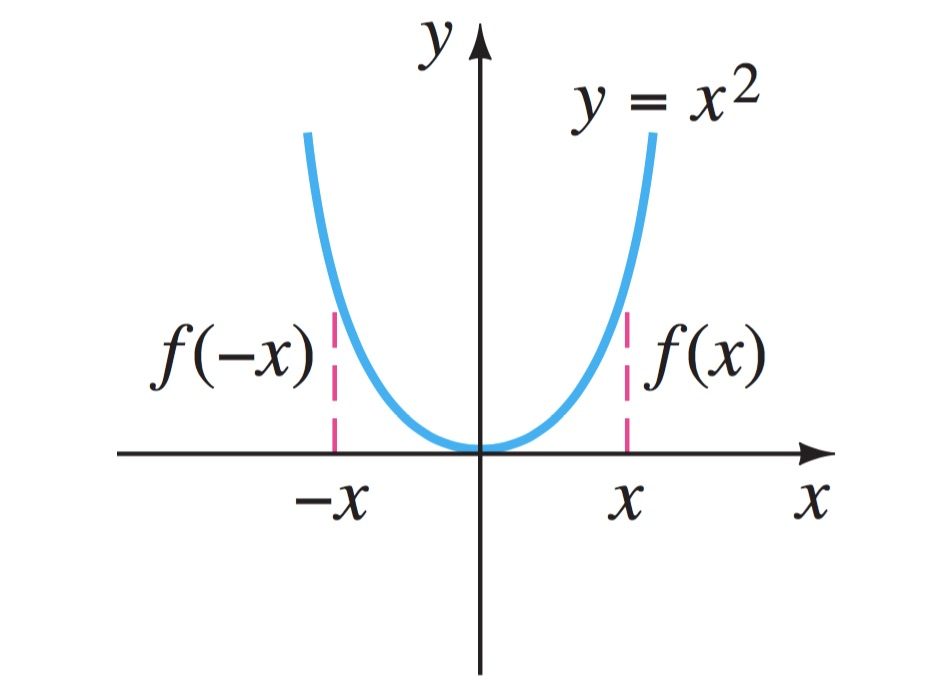
\includegraphics[width=3in]{evenFunction}
%\end{figure}
%\end{frame}
%%=-=-=-=-=-=-=-=-=-=-=-=-=-=-=-=-
%\subsection{Even and Odd Functions}
%\begin{frame}{Even and Odd Functions}
%It is likely that the origin of the terms even and odd derives from the fact that the graphs of polynomial functions that consist of all even powers of $x$ are symmetric with respect to the y-axis, whereas graphs of polynomials that consist of all odd powers of $x$ are symmetric with respect to origin. For example,
%\begin{eqnarray}
%  f(x)=x^2 \to f(-x)=(-x)^2=x^2=f(x)\nonumber\\
%  f(x)=x^3 \to f(-x)=(-x)^3=-x^3=-f(x)
%\end{eqnarray}
%\end{frame}
%%=-=-=-=-=-=-=-=-=-=-=-=-=-=-=-=-
%\begin{frame}{Odd function}
%  \begin{figure}
%    \includegraphics[width=3in]{oddFunction}
%  \end{figure}
%\end{frame}
%%=-=-=-=-=-=-=-=-=-=-=-=-=-=-=-=-
%\begin{frame}{Thus, Sine and Cosine...}
%  The trigonometric cosine and sine functions are even and odd functions, respectively, since $cos(-x)= cos(x)$ and $sin(-x)= -sin(x)$. The exponential functions $f(x)=e^x$ and $f(x)=  e^{-x}$ are neither odd nor even.
%\end{frame}
%%=-=-=-=-=-=-=-=-=-=-=-=-=-=-=-=-
%\begin{frame}{Properties of even and odd functions}
%\begin{theorem}{Properties of even and odd functions}
%  \begin{itemize}
%    \item The product of two even functions is even.
%    \item The product of two odd functions is even.
%    \item The product of an even function and an odd function is odd.
%    \item The sum (difference) of two even functions is even.
%    \item The sum (difference) of two odd functions is odd.
%    \item If $f$ is even, then $\int_{-a}^af(x)dx=2\int_{0}^af(x)dx$
%    \item If $f$ is odd,then $\int_{-a}^af(x)dx=0$
%  \end{itemize}
%\end{theorem}
%\end{frame}
%%-=-=-=-=-=-=-=-=-=-=-=-=-=-=-=
%\subsection{Half-range expansions}
%\begin{frame}{Half-range expansions}
%  \begin{exampleblock}{Exercise}
%  Expand $f(x)=x^2, 0<x<L$, in
%  \begin{enumerate}
%    \item a cosine series,
%    \item sine series and
%    \item Fourier series
%  \end{enumerate}
%  \end{exampleblock}
%\end{frame}
%--------------------
\begin{frame}{References}
	\begin{thebibliography}{10}
	\beamertemplatebookbibitems
  \bibitem{Nova2017}
  [1] Nova foundation for Science
  \newblock Pi \& the Fibonacci sequence
	\bibitem{Zill2009}
  [2] Deniss G. Zill and Michael R. Cullen
	\newblock Differential Equations with Boundary-Valuer Problems
	\bibitem{Math2017}
    [3] Math is Fun
	\newblock www.mathisfun.com

	\bibitem{Math242017}
    [4] Everything you need to master Calculus and Differential Equations
	\newblock www.math24.com

	\beamertemplatebookbibitems
	\bibitem{Swokowski1983}
	[5] Earl W. Swokowski
	\newblock Calculus with analytic geometry
	\newblock Prindle, Weber \& Schmidt, 1979

  \end{thebibliography}
\end{frame}
\end{document}
